\subsection{BBC Recipes}

\begin{figure}[h]
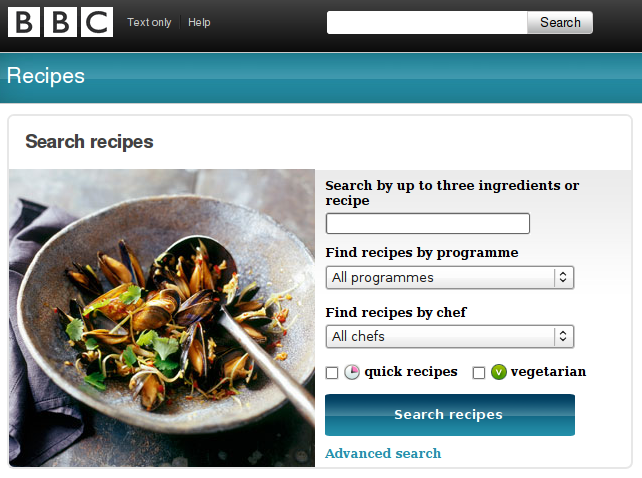
\includegraphics[width=0.9\textwidth]{screenshot_bbc_recipes}
\caption{The BBC Food Recipe Search Page}
\label{fig:bbc_food}
\end{figure}


BBC Recipes\footnote{[BBC Recipes, 24th November 2009 \url{www.bbc.co.uk/food/recipes/}]} (Fig~\ref{fig:bbc_food}) is a web application that allows the user to input up to three ingredients and returns a list of related recipes. 

BBC Recipes has two search options, basic and advanced. The basic search allows the user to input up to three ingredients with the option to find the recipe by television program or by chef. This search also provides the tagging options of quick recipes and vegetarian. However the advanced recipe search includes a wider choice of search preferences such as, the preparation method, cuisine, season and dietary requirements. After looking over the source code it’s very obvious that this web-based application uses an online database using a query language to return recipe results. 

One main attraction about this application is the advanced search option which includes a numerous amount of tag options. This option becomes quite useful when searching through a large database as this kind of search minimizes the results. A good example of this is a search including flour, butter and sugar with the season tag being ‘Christmas’ and the dietary needs tag being ‘nut-free’ returning only 14 recipes. However a search including just the three ingredients returns 400 recipes. 

However, the website has its flaws. For instance, the search field is a text box which takes text input, but does not validate the input until after the search. The validation matches the input with similar words, for example for ‘flor’ it will return ‘flour’. However not all typographical errors are corrected to the intended ingredient, which is a logical consequence using such a search methodology. For example typing ‘aooples’, instead of ‘apples’ returned the match ‘allows’. To solve this issue perhaps an automatic-complete feature could be implemented, where as the user types an igredient, the user is presented with a variety of completed strings from which he/she can choose allowed ingredients.

The design of the website is attractive with a good use of colour and images. However the navigation of the website is slightly tedious, the reason for this being when expanding the actual recipes on the home page the webpage’s content increases and therefore leaving the user to have to scroll through the webpage to view it’s content.

\subsection{RecipeZaar.com}

\begin{figure}[h]
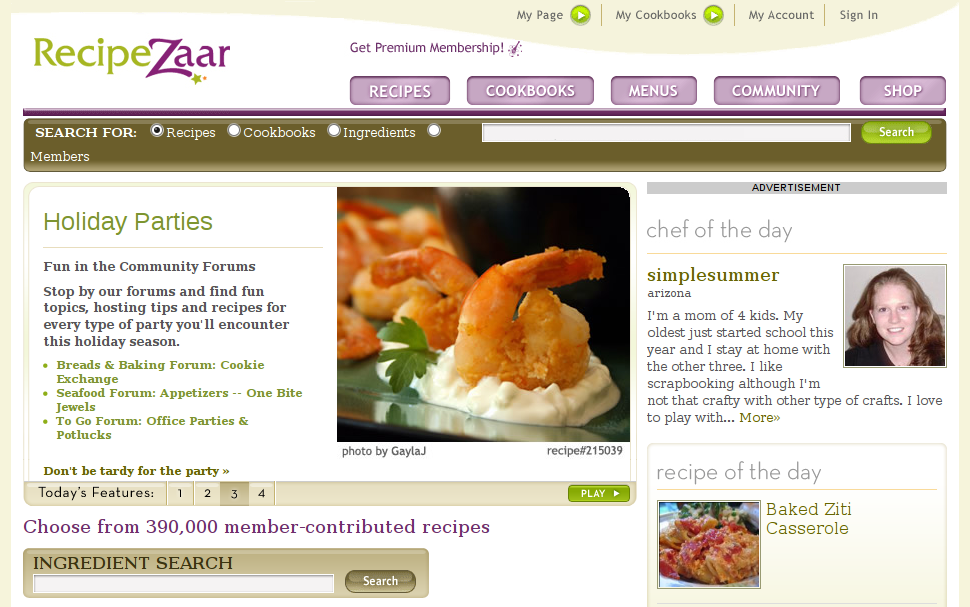
\includegraphics[width=0.9\textwidth]{screenshot_recipezaar}
\caption{The RecipeZaar.com Home Page}
\label{fig:recipezaar}
\end{figure}

Recipezaar\footnote{[ RecipeZaar, 24th November 2009 \url{https://RecipeZaar.com} ]} (Fig~\ref{fig:recipezaar}) is a website that includes a large database of recipes and user accounts. Recipes are searchable by recipes, cookbooks, ingredients and members. 

The recipe search allows the user to input $n$ number of ingredients. The input method is a text box which includes no validation. If the user inputs ‘flor’ instead of ‘flour’ the search returns nothing. Additionally, the query system used for search lacks intuition for inputs of many ingredients. For example if the user inputs ‘flour, sugar, butter, eggs’, the search asks users to refine their search by selecting from a generated list of more specific of ingredients. However, this returned list is extremely vague, mainly because users now have to select boxes such as ‘low-sugar apple butter’ (which, incredibly, was the first in the list) where the system combined the query for ‘butter’ and ‘sugar’. There is no checkbox for what one would have expected, like ‘granulated sugar’. Hence, such a system- where users have to input more specific ingredients before queries can be accepted- is ineffective for a search with many ingredients because the search now requires users to refine their search by selecting from a generated list which consists of mostly absurd ingredients (e.g. ‘sodium-free-sugar-free peanut butter’).
 
This website introduces the use of collaborative filtering, allowing users to rate recipes. Moreover, the website encourages social networking by allowing users to have user accounts where they do a variety of tasks, like submitting recipes. When viewing a member’s recipe there is also the option to send a private message, submit corrections, send the recipe to the users email address or mobile device and create a shopping list. The recipe page also directs the user to other recipes ‘like’ the chosen recipe. The website also has a community webpage with forums for general discussions. 

The interactive design of the website makes good use of JavaScript. The colour scheme is neutral with a good use of images.

\subsection{Supercook.com}

\begin{figure}[h]
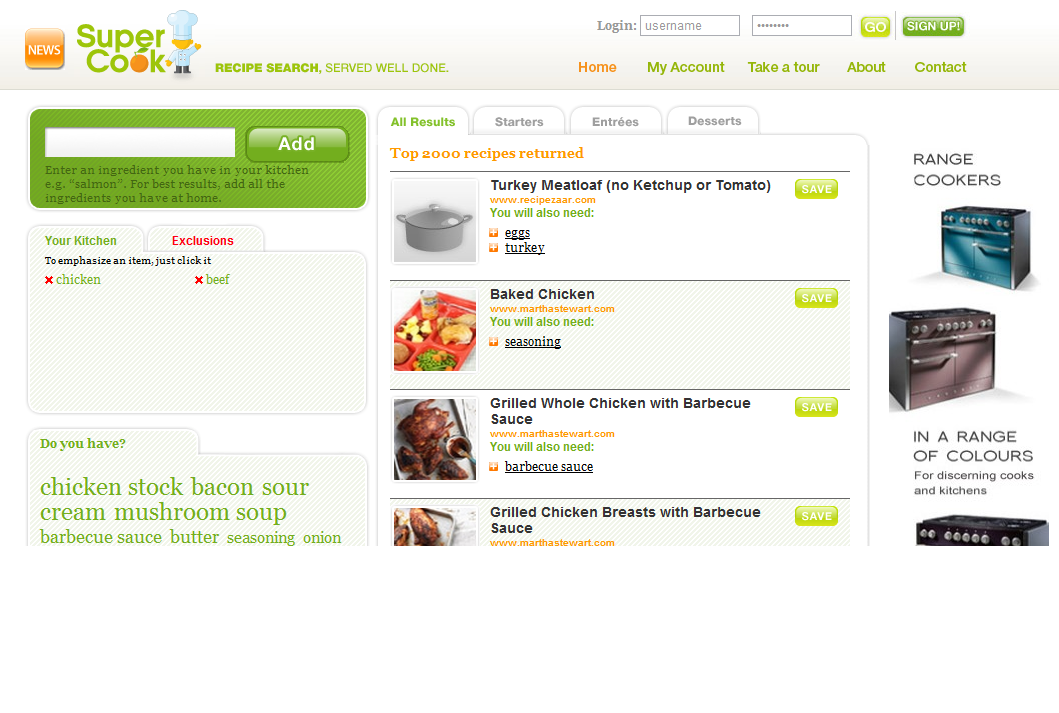
\includegraphics[width=0.9\textwidth]{screenshot_supercook}
\caption{The Supercook.com Home Page}
\label{fig:supercook}
\end{figure}

Supercook\footnote{[ Supercook, 17th February 2010 \url{https://Supercook.com} ]} (Fig~\ref{fig:supercook}) is one of the best websites surveyed due to its immense functionality and features. Its search-box has the automatic-complete feature, which validates user ingredients. Moreover, adding multiple ingredients is done by putting the ingredients in a list one at a time on the left side of the page, while recipe results are seamlessly displayed on the right hand side of the page as ingredients are added.

The results also inform you if you have all the ingredients you need to make the recipe. In case you do not, the returned recipe tells you what additional materials you will need in a very user friendly format. Moreover, there is a ‘do you have’ area where if you have the additional ingredient displayed, then you can make a recipe without needing extra materials. This is useful because it provides a way for users to find potentially unique combinations of ingredients to complete a recipe based on the suggestion, which they would otherwise not have thought of. 

You can also specify what ingredients to exclude in the search. For example, you may wish to exclude ‘milk’ from the returned recipes if you are lactose intolerant.

Another atypical feature about this website is that the returned recipes are actually links to other websites, like recipezaar.com. So clicking a recipe results in redirection to another website. This introduces a problem of standards, because each website linked has its own way of displaying recipes, and the level of detail for the instructions. An improvement would have been for supercook.com to use its own database.

Moreover, the website is quite chaotic in its layout. The most jarring are the advertisements which occupy multiple areas on the webpage as opposed to a fixed area.

\subsection{Allrecipes.com}

\begin{figure} [h]
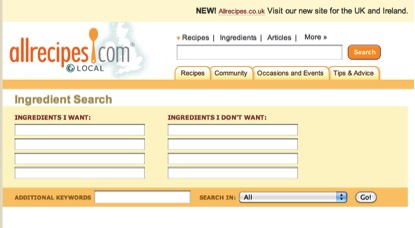
\includegraphics[width=0.9\textwidth]{allrecipes}
\caption{The Allrecipes.com Home Page}
\label{fig:allrecipes}
\end{figure}

Allrecipes\footnote{[ Allrecipes, 23rd March 2010 \url{http://allrecipes.com} ]} (Fig~\ref{fig:allrecipes}) is a web application that allows the user to search for recipes using four ingredients they wish to search by, and four ingredients that they don�t wish to search by. There�s also the additional feature to add keywords and the ability to search using different tags, for example, Asian, breakfast and brunch, seafood etc� 

Recipes are returned and sorted by relevance, title or ratings. Each recipe has a rating, reviews and the ability to find recipes like the recipe chosen. The users submit the recipes including details such as, the prep time for the recipe, the cook time, the ready in time, servings, ingredients and directions.
 
Each user has a user account. The user account includes the users home town, where they�re currently living, the length of time that they�ve been a member, their cooking level, interests such as baking, Indian, Italian etc, cooks that they like, a recipe box, a blog and an about section. 
 
This website has a good use of collaborative filtering. The colours used and the design of the website is minimum. The simplicity of the website allows the users to navigate freely. With the use of �recipe of the day � this gives the user reason to revisit the website on a regular basis. 


\subsection{JamieOliver.com}

%need to upload image%
JamieOliver\footnote{[ JamieOliver, 23rd March 2010 \url{http://www.jamieoliver.com} ]}
This website allows the user to search for recipes rather than inputting ingredients. The website returns a list of recipes meeting the text inputted into the search field.  A recipe consists of ingredients and directions. This website doesn�t use collaborative filtering as well as other recipe websites, however does include recipe comments, blogs and user profiles.  

The overall design of this website is very attractive and has a good use of colours that really catch the eye. With the use of a slide show this makes the website more interactive. 


\subsection{Jamie Oliver - 20 Minute Meals Iphone Application}

%need to upload image%

This application provides a list of recipes. Dishes include easy pasta, delicious soups, fast fish and many more. It then provides the user with a summary of the chosen recipe, ingredients that you�ll need and the steps to follow. The images used look very appetising and �handy videos� are also available. 

The application also provides the user with the capability of creating a shopping list using ingredients from the recipes and also adding their own shopping items. 








